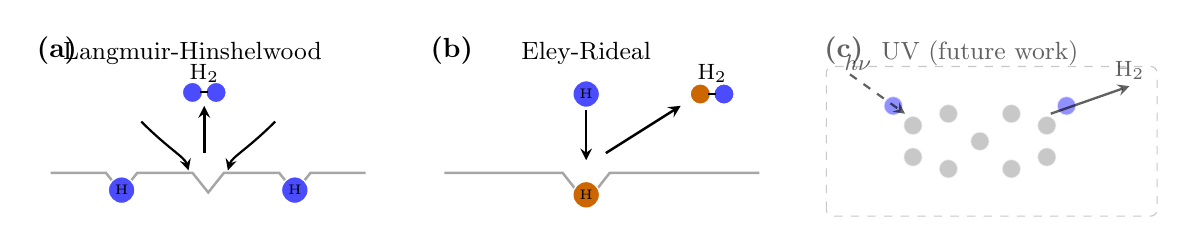
\begin{tikzpicture}[x=1cm,y=1cm,>=stealth]
\tikzstyle{surface}=[line width=0.9pt, draw=gray!70]
\tikzstyle{atom}=[circle, draw=white, line width=0.5pt, minimum size=0.34cm, inner sep=0pt]
\tikzstyle{labeltext}=[font=\footnotesize]
\tikzstyle{paneltitle}=[font=\small]

% Panel A
\begin{scope}[shift={(0,0)}]
  \node[anchor=west,font=\bfseries] at (0.0,2.25) {(a)};
  \node[paneltitle] at (2.1,2.22) {Langmuir-Hinshelwood};
  \draw[surface] (0.3,0.7)--(1.0,0.7)--(1.2,0.45)--(1.4,0.7)--(2.1,0.7)--(2.3,0.45)--(2.5,0.7)--(3.2,0.7)--(3.4,0.45)--(3.6,0.7)--(4.3,0.7);
  \node[atom, fill=blue!70] (h1) at (1.2,0.48) {\tiny H};
  \node[atom, fill=blue!70] (h2) at (3.4,0.48) {\tiny H};
  \draw[->, line width=0.8pt] (1.45,1.35) .. controls (1.8,1.0) and (2.0,0.9) .. (2.05,0.73);
  \draw[->, line width=0.8pt] (3.15,1.35) .. controls (2.8,1.0) and (2.6,0.9) .. (2.55,0.73);
  \draw[->, line width=0.9pt] (2.25,0.95) -- (2.25,1.55);
  \node[atom, fill=blue!70, minimum size=0.26cm] at (2.1,1.72) {};
  \node[atom, fill=blue!70, minimum size=0.26cm] at (2.4,1.72) {};
  \draw[line width=0.7pt] (2.2,1.72)--(2.3,1.72);
  \node[labeltext] at (2.25,1.96) {H$_2$};
\end{scope}

% Panel B
\begin{scope}[shift={(5.0,0)}]
  \node[anchor=west,font=\bfseries] at (0.0,2.25) {(b)};
  \node[paneltitle] at (2.1,2.22) {Eley-Rideal};
  \draw[surface] (0.3,0.7)--(1.8,0.7)--(2.1,0.32)--(2.4,0.7)--(4.3,0.7);
  \node[atom, fill=orange!80!black] (hs) at (2.1,0.42) {\tiny H};
  \node[atom, fill=blue!70] (hg) at (2.1,1.7) {\tiny H};
  \draw[->, line width=0.85pt] (2.1,1.5)--(2.1,0.86);
  \draw[->, line width=0.9pt] (2.35,0.95) -- (3.3,1.55);
  \node[atom, fill=orange!80!black, minimum size=0.26cm] at (3.55,1.7) {};
  \node[atom, fill=blue!70, minimum size=0.26cm] at (3.85,1.7) {};
  \draw[line width=0.7pt] (3.65,1.7)--(3.75,1.7);
  \node[labeltext] at (3.7,1.96) {H$_2$};
\end{scope}

% Panel C
\begin{scope}[shift={(10.0,0)}, opacity=0.62]
  \node[anchor=west,font=\bfseries] at (0.0,2.25) {(c)};
  \node[paneltitle] at (2.1,2.22) {UV (future work)};
  \draw[rounded corners=0.08cm, dashed, draw=gray!70] (0.15,0.15) rectangle (4.35,2.05);
  \foreach \x/\y in {2.1/1.1,1.7/1.45,1.25/1.3,1.25/0.9,1.7/0.75,2.5/0.75,2.95/0.9,2.95/1.3,2.5/1.45}
    \node[atom, fill=gray!70, minimum size=0.24cm] at (\x,\y) {};
  \node[atom, fill=blue!70, minimum size=0.24cm] at (1.0,1.55) {};
  \node[atom, fill=blue!70, minimum size=0.24cm] at (3.2,1.55) {};
  \draw[->, dashed, line width=0.8pt] (0.45,1.95) -- (1.15,1.45);
  \node[labeltext] at (0.55,2.1) {$h\nu$};
  \draw[->, line width=0.85pt] (3.0,1.45) -- (4.0,1.8);
  \node[labeltext] at (4.0,2.0) {H$_2$};
\end{scope}
\end{tikzpicture}

